\documentclass[14pt, a4paper]{extarticle}
\usepackage{GOST}
\usepackage{array}
\usepackage{verbatim}
\usepackage[detect-all]{siunitx}
\usepackage{amsmath}
\usepackage{amssymb}
\usepackage[utf8]{inputenc}
\usepackage{hyperref}

\usepackage{ifthen}

\makeatletter
\renewcommand\@biblabel[1]{#1.}
\makeatother

\usepackage{listings}
\lstset{ 
	language=python,
	basicstyle=\small\sffamily, 
	numbers=left, 
	numberstyle=\tiny,
	stepnumber=1,
	numbersep=5pt,
	showspaces=false,            
	showstringspaces=false,      
	showtabs=false,             
	frame=single,            % рисовать рамку вокруг кода
	tabsize=4,      
	commentstyle=\color{green},
	keywordstyle=\color{blue}\textbf,
	numberstyle=\scriptsize\color{gray}, % the style that is used for the line-numbers
	rulecolor=\color{black},
	captionpos=t,
	breaklines=true,         % автоматически переносить строки 
	breakatwhitespace=false, % переносить строки по пробелу
	escapeinside={\#*}{*)} 
}


\usepackage{pgfplots}
\usepackage{filecontents}
\usetikzlibrary{datavisualization}
\usetikzlibrary{datavisualization.formats.functions}

\begin{document}
	
\begin{table}[ht]
	\centering
	\begin{tabular}{|c|p{400pt}|} 
		\hline
		\begin{tabular}[c]{@{}c@{}} 
\includegraphics[scale=1]{source/b_logo.jpg} \\\end{tabular} &
		\footnotesize\begin{tabular}[c]{@{}c@{}}\textbf{Министерство~науки~и~высшего~образования~Российской~Федерации}\\\textbf{Федеральное~государственное~бюджетное~образовательное~учреждение}\\\textbf{~высшего~образования}\\\textbf{«Московский~государственный~технический~университет}\\\textbf{имени~Н.Э.~Баумана}\\\textbf{(национальный~исследовательский~университет)»}\\\textbf{(МГТУ~им.~Н.Э.~Баумана)}\\\end{tabular}  \\
		\hline
	\end{tabular}
\end{table}
\noindent\rule{\textwidth}{4pt}
\noindent\rule[14pt]{\textwidth}{1pt}
\hfill 
\noindent
\makebox{ФАКУЛЬТЕТ~}%
\makebox[\textwidth][l]{\underline{~«Информатика и системы управления»~~~~~~~~~~~~~~~~~~~~~~~~~~~~~~~~~}}%
\\
\noindent
\makebox{КАФЕДРА~}%
\makebox[\textwidth][l]{\underline{~«Программное обеспечение ЭВМ и информационные технологии»~}}%
\\

\begin{center}
	\vspace{1.5cm}
	{\bf\huge Отчёт\par}
	{\bf\Large по лабораторной работе № 3\par}
	\vspace{0.7cm}
\end{center}


\noindent
\makebox{\large{\bf Название:}~~~}
\makebox[\textwidth][l]{\large\underline{~Алгоритмы сортировки~~~~~~~~~~~~~}}\\

\noindent
\makebox{\large{\bf Дисциплина:}~~~}
\makebox[\textwidth][l]{\large\underline{~Анализ алгоритмов~~~~~~~~~~~~~~~~~~~~~~~~~~}}\\

\vspace{1.5cm}
\noindent
\begin{tabular}{l c c c c c}
	Студент      & ~ИУ7-55Б~               & \hspace{2.5cm} & \hspace{2cm}                 & &  Д.О. Склифасовский \\\cline{2-2}\cline{4-4} \cline{6-6} 
	\hspace{3cm} & {\footnotesize(Группа)} &                & {\footnotesize(Подпись, дата)} & & {\footnotesize(И.О. Фамилия)}
\end{tabular}

\noindent
\begin{tabular}{l c c c c}
	Преподователь & \hspace{5cm}   & \hspace{2cm}                 & & ~~~~~~Л.Л. Волкова~~~~~~\\\cline{3-3} \cline{5-5} 
	\hspace{3cm}  &                & {\footnotesize(Подпись, дата)} & & {\footnotesize(И.О. Фамилия)}
\end{tabular}

\vspace{0.6cm}
\begin{center}	
	\vfill
	\large \textit {Москва, 2020}
\end{center}

\thispagestyle {empty}
\pagebreak

% СОДЕРЖАНИЕ 
\clearpage
\tableofcontents


% ВВЕДЕНИЕ
\clearpage
\section*{Введение}
\addcontentsline{toc}{section}{Введение}
Цель работы: изучение алгоритмов сортировки массивов. В данной лабораторной работе рассматриваются 3 алгоритма:
\begin{enumerate}
	\item[1)] сортировка пузырьком;
	\item[2)] сортировка выбором;
	\item[3)] сортировка вставками. 
\end{enumerate}\par
Также требуется изучить рассчет сложности алгоритмов. В ходе лабораторной работы необходимо:
\begin{enumerate}
	\item[1)] изучить алгоритмы сортировки;
	\item[2)] дать теоритическую оценку сортировок пузырьком, шейкером и вставками;
	\item[3)] реализовать три алгоритма сортировки на одном из языков программирования;
	\item[4)] сравнить алгоритмы сортировки.    
\end{enumerate}

% АНАЛИТИЧЕСКИЙ РАЗДЕЛ
\clearpage
\section{Аналитический раздел}
В данном разделе представлено описание алгоритмов сортировки массивов.\hyperref[literature]{[1]}
\subsection{Сортировка пузырьком}
Сортировка пузырьком — один из самых известных алгоритмов сортировки. Здесь нужно последовательно сравнивать значения соседних элементов и менять числа местами, если предыдущее оказывается больше последующего. Таким образом элементы с большими значениями оказываются в конце списка, а с меньшими остаются в начале.\par
Этот алгоритм считается учебным и почти не применяется на практике из-за низкой эффективности: он медленно работает на тестах, в которых маленькие элементы (их называют «черепахами») стоят в конце массива. Однако на нём основаны многие другие методы, например, шейкерная сортировка и сортировка расчёской.
\subsection{Сортировка выбором}
В сортировке выбором мы целенаправленно ищем максимальный элемент (или минимальный), которым дополняем отсортированную часть массива.
\subsection{Сортировка вставками}
При сортировке вставками массив постепенно перебирается слева направо. При этом каждый последующий элемент размещается так, чтобы он оказался между ближайшими элементами с минимальным и максимальным значением.
\subsection{Вывод}
Было представлено описание алгоритмов сортировки массивов. В основном все алгоритмы сортировок основаны на алгоритме сортировки пузырьком.

%КОНСТРУКТОРСКИЙ РАЗДЕЛ
\clearpage
\section{Конструкторский раздел}
В данном разделе представлены съемы разработанных алгоритмов. Также оценивается трудоемкость алгоритмов.
\subsection{Разработка алгоритмов}
На \hyperref[Schema1]{рисунке 1} изображена схема алгоритма сортировки пузырьком.
\begin{figure}[h!]
	\centering
	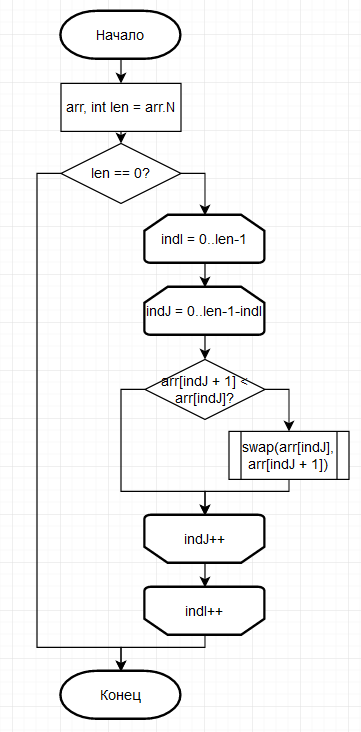
\includegraphics[height=0.7\textheight]{source/Schema1.png}
	\caption{Схема алгоритма сортировки пузырьком}
	\label{Schema1}
\end{figure}
\clearpage
На \hyperref[Schema2]{рисунке 2} изображена схема алгоритма сортировки выбором.
\begin{figure}[h!]
	\centering
	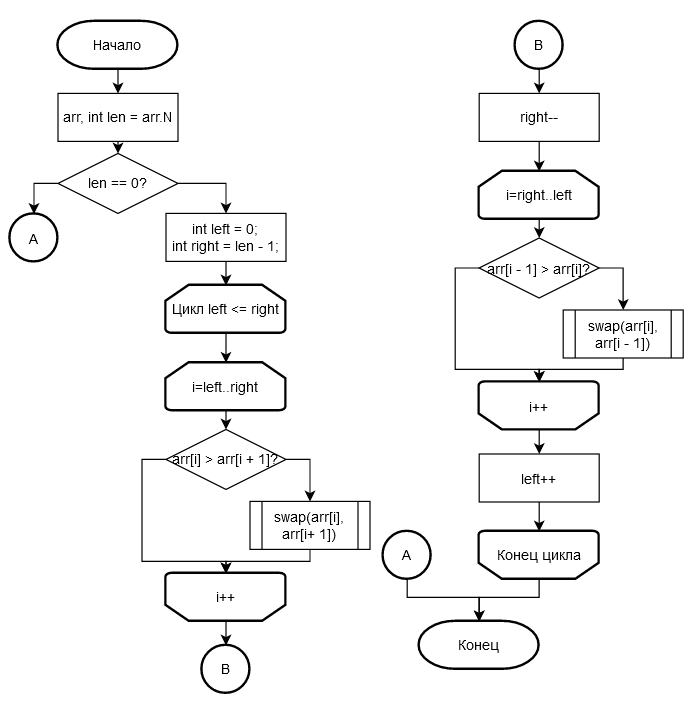
\includegraphics[height=0.7\textheight]{source/Schema2.png}
	\caption{Схема алгоритма сортировки выбором}
	\label{Schema2}
\end{figure}
\clearpage
На \hyperref[Schema3]{рисунке 3} изображена схема алгоритма сортировки вставками.
\begin{figure}[h!]
	\centering
	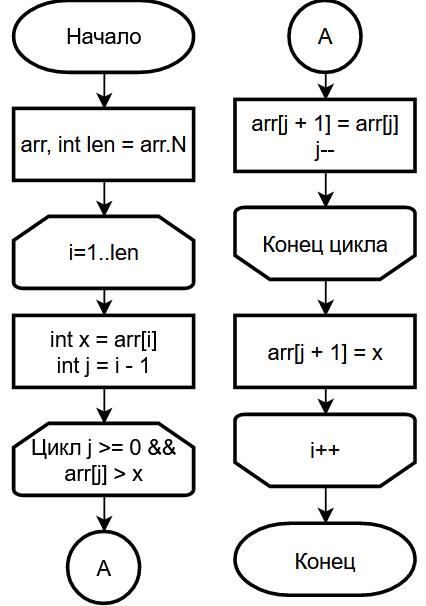
\includegraphics[height=0.7\textheight]{source/Schema3.png}
	\caption{Схема алгоритма сортировки вставками}
	\label{Schema3}
\end{figure}	
\subsection{Модель трудоемкости}
Модель трудоемкости для оценки алгоритмов:
\begin{enumerate}
	\item[1)] стоимость базовых операций единица:\par
	$=,+,*,\simeq,<,>,\geq,\leq,==,!=,[],+=,-=,*=,/=,++,--$;
	\item[2)] стоимость цикла:\par
	$f_{for}=f_{init}+f_{comp}+M(f_{body}+f_{increment}+f_{comp})$\par
	Пример: $for(i=0,i<M;i++){/* body */}$\par
	Результат: $2 + M(2+f_{body})$;
	\item[3)] стоимость условного оператора\par
	Пусть goto (переход к одной из ветвей) стоит 0, тогда\par
	\begin{displaymath}
		f_{f} = \left\{ \begin{array}{l l}
			min(f_{A},f_{B}), & \textrm{лучший случай}\\
			max(f_{A},f_{B}), & \textrm{худший случай}\\
		\end{array} \right.
	\end{displaymath}
	\item[4)] операция обращения к ячейки матрицы [i, j] имеет трудоёмкость равную двум.
\end{enumerate}

\subsection{Оценка трудоемкости алгоритмов сортировки}
Оценим трудоемкость алгоритмов.\par
\vspace{\baselineskip}
\noindent\textbf{Трудоемкость функции Swap}\par
\begin{displaymath}
	f_{swap}=2+3+3=8
\end{displaymath}\par

\vspace{\baselineskip}
\noindent\textbf{Сортировка пузырьком}\par
Внутренний цикл будет выполняться: $n-0-1,n-1-1,n-2-1,...,n-(n-2)-1$ раз. Эта последовательность является арифметической прогрессией и ее можно записать как:\par
\begin{displaymath}
	s_{bubble}=\frac{(n-1)n}{2}
\end{displaymath}\par
\textbf{Лучший случай} (массив отсортирован): $f_{bubble} = 2 + (3+4+(n-0-1)(4+4)) + (4+3+(n-1-1)(4+4)) + ... + (4+3+(n-(n-2)-1)(4+4)) = 2+7(n-1)+8s_{bubble}=2+7(n-1)+8\frac{(n-1)n}{2}=4n^2+3n-5 \thickapprox 4n^2$\par
\textbf{Худший случай} (массив отсортирован в порядке, обратном нужному, т.е. каждый раз будет выполняться тело условного оператора): $f_{bubble}=3+(3+4+(n-0-1)(4+4+f_{swap}))+(3+4+(n-1-1)(4+4+f_{swap}))+...+(3+4+(n-(n-2)-1)(4+4+f_{swap})) = 3+7(n-1)+15s_{bubble}=3+7(n-1)+15\frac{(n-1)n}{2} \thickapprox \frac{15}{2}n^2$\par

\vspace{\baselineskip}
\noindent\textbf{Сортировка выбором}\par
Внутренний цикл будет выполняться: $n-1,n-2,n-3,...,n-(n-1)$ раз. Эта последовательность является арифметической прогрессией и ее можно записать как:\par
\begin{displaymath}
	s_{selection}=\frac{(n-1)n}{2}
\end{displaymath}\par
\textbf{Лучший случай} (массив отсортирован): $f_{selection}=3+(3+1+3+(n-1)(2+3)+2+f_{swap})+(3+1+3+(n-2)(2+3)+2+f_{swap})+...+(3+1+3+(n-(n-1))(2+3)+2+f_{swap})=3+12(n-1)+12(n-1)+5*s_{selection}=\frac{5}{2}n^2+9n-9 \thickapprox \frac{5}{2}n^2$\par
\textbf{Худший случай} (массив отсортирован в порядке, обратном нужному, т.е. каждый раз будет выполняться тело условного оператора): $f_{selection} = 3+(3+1+3+(n-1)(2+3+1)+2+f_{swap}) + (3+1+3+(n-2)(2+3+1)+2+f_{swap}) + ... + (3+1+3+(n-(n-1))(2+3+1)+2+f_{swap}) = 3+12(n-1)+6s_{selection}=3n^2+8n-8 \thickapprox 3n^2$\par

\vspace{\baselineskip}
\noindent\textbf{Сортировка вставками}\par
Внутренний цикл будет выполняться: $1,2,3,...,n-1$ раз. Эта последовательность является арифметической прогрессией и ее можно записать как:\par
\begin{displaymath}
	s_{insert}=\frac{(n-1)n}{2}
\end{displaymath}\par
\textbf{Лучший случай} (массив отсортирован): $f_{insertion}=2+(n-1)(2+2+2+4+3)=13n-11 \thickapprox 13n$\par
\textbf{Худший случай} (массив отсортирован в порядке, обратном нужному, т.е. каждый раз будет выполняться тело условного оператора): $f_{insertion}=2+(2+2+4+1(5+4)+3)+(2+2+4+2(5+4)+3)+...+(2+2+4+(n-1)(5+4)+3) = 2+11(n-1)+9*s_{insert}=\frac{9}{2}n^2+\frac{13}{2}n-9 \thickapprox \frac{9}{2}n^2$\par

\subsection{Вывод}
В данном разделе были рассмотрены схемы алгоритмов сортировки массива, введена модель оценки трудоемкости алгоритма и были рассчитаны трудоемкости алгоритмов.

\clearpage
%ТЕХНОЛОГИЧЕСКИЙ РАЗДЕЛ
\section{Технологический раздел}
В данном разделе даны общие требования к программе, средства реализации и реализация алгоритмов.

\subsection{Общие требования к программе}
\textbf{Требования к вводу:}
\begin{enumerate}
	\item[1)] вводится размер массива;
	\item[2)] вводятся или автоматически генерируется массив. 
\end{enumerate}
\textbf{Требования к программе:}
\begin{enumerate}
	\item[1)] при вводе неправильных размеров массива программа не должна завершаться аварийно;
	\item[2)] должна выполняться корректная сортировка массива. 
\end{enumerate}

\subsection{Средства реализации}
В качестве языка программирования был выбран C\#\hyperref[literature]{[2]}, так как я знаком с данным языком программирования, имею представление о способах тестирования программы.
\noindent Средой разработки Visual Studio.\hyperref[literature]{[3]}
\noindent Для замеров процессорного времени используется функция Stopwatch.\hyperref[literature]{[4]}\hyperref[literature]{[5]}

\subsection{Сведения о модулях программы}
Программа состоит из:
\begin{enumerate}
	\item[1)] Program.cs - главный файл программы, в котором располагается точка входа в программу;
	\item[2)] Array.cs - файл класса Array;
	\item[3)] Sort.cs - файл класса Sort. В нем находятся алгоритмы сортировки массивов.
\end{enumerate}

\subsection{Листинг кода программы}
В листинге 1 реализован класс Array. Он используется для работы с массивами.
\begin{lstlisting}[label=Array,caption=Класс Array для работы с массивами]
	class Array
	{
		private int[] array;
		private int n;
		public Array() { }
		
		public Array(int n)
		{
			this.n = n;
			array = new int[n];
		}
		
		public int N
		{
			get { return n; }
			set { if (value > 0) n = 0; }
		}
		
		public int this[int i]
		{
			get { return array[i]; }
			set { array[i] = value; }
		}
		
		public void Copy(Array arr)
		{
			for (int i = 0; i < n; i++)
			{
				arr[i] = array[i];
			}
		}
		
		public void Read()
		{
			for (int i = 0; i < n; i++)
			{
				Console.Write(array[i] + "\t");
			}
			Console.WriteLine();
		}
		
		public void Fill()
		{
			Random rand = new Random();
			for (int i = 0; i < n; i++)
			{
				array[i] = rand.Next(100);
			}
		}
	}
\end{lstlisting}
В листинге 2 реализован алгоритм сортировки пузырьком.
\begin{lstlisting}[label=BubleSort,caption=Алгоритм сортировки пузырьком]
	public static void BubbleSort(Array arr)
	{
		int len = arr.N;
		for (int indI = 0; indI + 1 < len; indI++)
		{
			for (int indJ = 0; indJ + 1 < len - indI; indJ++)
			{
				if (arr[indJ + 1] < arr[indJ])
				{ 
					int tmp = arr[indJ];
					arr[indJ] = arr[indJ + 1];
					arr[indJ + 1] = tmp;
				}
			}
		}
	}
\end{lstlisting}
В листинге 3 реализован алгоритм сортировки выбором.
\begin{lstlisting}[label=SelectionSort,caption=Алгоритм сортировки выбором]
	public static void SelectionSort(Array arr)
	{
		int len = arr.N;
		for (int i = 0; i < len - 1; i++)
		{
			int select = i;
			for (int j = i + 1; j < len; j++)
			{
				if (arr[j] < arr[select])
				{
					select = j;
				}
				
			}
			int tmp = arr[select];
			arr[select] = arr[i];
			arr[i] = tmp;
		}
	}
\end{lstlisting}
В листинге 4 реализован алгоритм сортировки вставками.
\begin{lstlisting}[label=InsertionSort,caption=Алгоритм сортировки вставками]
	public static void InsertionSort(Array arr)
	{
		int len = arr.N;
		for (int i = 1; i < len; i++)
		{
			int x = arr[i];
			int j = i - 1;
			for (; j >= 0 && arr[j] > x; j--)
			{
				arr[j + 1] = arr[j];
			}
			arr[j + 1] = x;
		}
	}
\end{lstlisting}

\subsection{Вывод}
В данном разделе были представлены сведения о модулях программы, а также реализованы три алгоритма сортировки массивов.

%ЭКСПЕРИМЕНТАЛЬНЫЙ РАЗДЕЛ
\clearpage
\section{Экспериментальный раздел}
В данном разделе представлены результаты работы программы и приведен анализ времени работы каждого из алгоритмов.
\subsection{Примеры работы программы}
На \hyperref[Result1]{рисунке 4} представлен результат работы алгоритмов.
\begin{figure}[h!]
	\centering
	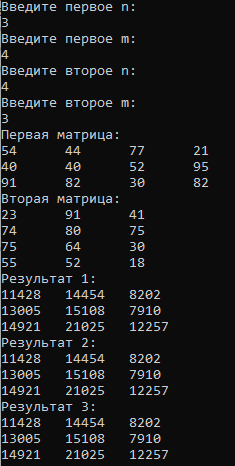
\includegraphics[scale=0.9]{source/Result1.png}
	\caption{Первый результат работы программы}
	\label{Result1}
\end{figure}\par
На \hyperref[Result2]{рисунке 5} представлен результат работы алгоритмов.
\begin{figure}[h!]
	\centering
	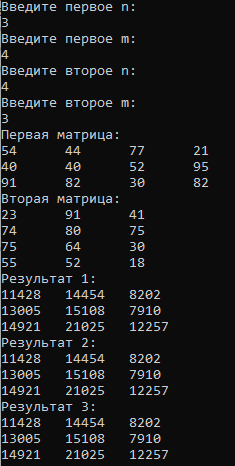
\includegraphics[scale=0.9]{source/Result1.png}
	\caption{Второй результат работы программы}
	\label{Result2}
\end{figure}
\clearpage
\subsection{Анализ времени работы алгоритмов}
Выполняется первый эксперимент. Берутся заранее отсортированные масивы размерами 100, 200, 300, 400 и 500. Элементы массива заполняются произвольно. Результат можно увидеть на \hyperref[Graph1]{рисунке 6}.
\begin{figure}[h!]
	\centering
	\begin{tikzpicture}[object/.style={thin,double,<->}]
		
		\begin{axis}[
			axis lines = left,
			xlabel = $\textit{размер массива}$,
			ylabel = {$\textit{время сортировки, тики.}$},
			legend pos=north west,
			ymajorgrids=true
			]
			\addplot[color=red] table[x index=0, y index=1] {dat/buGood.dat}; 
			\addplot[color=orange] table[x index=0, y index=1] {dat/seGood.dat};
			\addplot[color=blue, mark=square] table[x index=0, y index=1] {dat/inGood.dat};
			
			\addlegendentry{Сортировка пузырьком}
			\addlegendentry{Сортировка выбором}
			\addlegendentry{Сортировка вставками}
			
		\end{axis}
	\end{tikzpicture}
	
	\caption{Результаты замеров процессорного времени сортировки уже упорядоченных массивов.}
	\label{Graph1}
\end{figure}
\clearpage
Выполняется второй эксперимент. Берутся заранее отсортированные в обратном порядке масивы размерами 100, 200, 300, 400 и 500. Элементы массива заполняются произвольно. Результат можно увидеть на \hyperref[Graph2]{рисунке 7}.
\begin{figure}[h!]
	\centering
	\begin{tikzpicture}[object/.style={thin,double,<->}]
		
		\begin{axis}[
			axis lines = left,
			xlabel = $\textit{размер массива}$,
			ylabel = {$\textit{время сортировки, тики.}$},
			legend pos=north west,
			ymajorgrids=true
			]
			\addplot[color=red] table[x index=0, y index=1] {dat/buBad.dat}; 
			\addplot[color=orange] table[x index=0, y index=1] {dat/seBad.dat};
			\addplot[color=blue, mark=square] table[x index=0, y index=1] {dat/inBad.dat};
			
			\addlegendentry{Сортировка пузырьком}
			\addlegendentry{Сортировка выбором}
			\addlegendentry{Сортировка вставками}
			
		\end{axis}
	\end{tikzpicture}
	
	\caption{Результаты замеров процессорного времени сортировки массивов, отсортированных в обратном порядке.}
	\label{Graph2}
\end{figure}
\clearpage
Выполняется третий эксперимент. Берутся масивы с произвольным порядком и размерами 100, 200, 300, 400 и 500. Элементы массива заполняются произвольно. Результат можно увидеть на \hyperref[Graph3]{рисунке 8}.
\begin{figure}[h!]
	\centering
	\begin{tikzpicture}[object/.style={thin,double,<->}]
		
		\begin{axis}[
			axis lines = left,
			xlabel = $\textit{размер массива}$,
			ylabel = {$\textit{время сортировки, тики.}$},
			legend pos=north west,
			ymajorgrids=true
			]
			\addplot[color=red] table[x index=0, y index=1] {dat/buRand.dat}; 
			\addplot[color=orange] table[x index=0, y index=1] {dat/seRand.dat};
			\addplot[color=blue, mark=square] table[x index=0, y index=1] {dat/inRand.dat};
			
			\addlegendentry{Сортировка пузырьком}
			\addlegendentry{Сортировка выбором}
			\addlegendentry{Сортировка вставками}
			
		\end{axis}
	\end{tikzpicture}
	
	\caption{Результаты замеров процессорного времени сортировки массивов.}
	\label{Graph3}
\end{figure}

\subsection{Вывод}
Результаты тестирования показывают, что во всех трес случаях порядка массива самым быстрым является алгоритм сортировки вставками. Самым медленным оказался алгоритм сортировки пузырьком. Сортировка выбором немного медленнее, чем сортировка вставками, в случаях упорядоченного и неупорядоченного заполнения массива. В случае обратного порядка массива - время работы сортировки выбором схоже с временем работы сортировки вставками.

\clearpage
\subsection*{Заключение}
\addcontentsline{toc}{section}{Заключение}
В ходе выполнения лабораторной работы были изучены алгоритмы сортировки массивов: пузырьком, выбором и вставками. Были даны теоритические оценки алгоритмов умножения матриц. Была оценена трудоемкость алгоритмов. Также сравнили время работы алгоритмов, в результате которого стало понятно, что алгоритм сортировки вставками примерно в 3 раза эффективнее по времени сортировки пузырьком и в 1.5 раза быстрее, что сортировка выбором.

\clearpage
\section*{Литература}
\addcontentsline{toc}{section}{Литература}
\begin{enumerate}
	\label{literature}
	\item Описание алгоритмов сортировки и сравнение их производительности. -URL: \href{https://habr.com/ru/post/335920/}{https://habr.com/ru/post/335920/} (дата обращения: 22.10.2020). -Текст: электронный.
	\item  Документация по C\#. -URL: \href{https://docs.microsoft.com/ru-ru/dotnet/csharp/}{https://docs.microsoft.com/ru-ru/dotnet/csharp/} (дата обращения: 01.10.2020). -Текст: электронный.
	\item Документация по семейству продуктов Visual Studio. -URL:\par \href{https://docs.microsoft.com/ru-ru/visualstudio/?view=vs-2019}{https://docs.microsoft.com/ru-ru/visualstudio/?view=vs-2019 } (дата обращения: 01.10.2020). -Текст: электронный.
	\item Stopwatch Класс. -URL: \href{https://goo.su/2e99}{https://goo.su/2e99 } (дата обращения: 01.10.2020). -Текст: электронный.
	\item Под капотом у Stopwatch. -URL:  \href{https://habr.com/ru/post/226279/}{https://habr.com/ru/post/226279/} (дата обращения: 01.10.2020). Текст: электронный.
\end{enumerate}
\end{document}\par